%% ============================================================================
%%  VeriCon: Mining, Falsifying, and Injecting Configuration Constraints
%%  for LLM Inference Engines
%%
%%  Target venue: IEEE Transactions on Software Engineering (TSE)
%%  Format: IEEEtran journal class (two-column)
%%  Compile: pdflatex main  (or upload the latex/ folder to Overleaf)
%%  Figures: ./figs/fig{1..9}.pdf
%%
%%  Notes for the author (delete before submission if desired):
%%   - Author info filled (Shuheng Zhao, zshbdfdc@163.com, September 28, 2026).
%%   - All numbers are traceable to the released artifact directory (Appendix A).
%%   - Bibliography is inlined (no BibTeX run required) for robustness.
%% ============================================================================
\documentclass[journal]{IEEEtran}

\usepackage{graphicx}
\usepackage{booktabs}
\usepackage{amsmath,amssymb}
\usepackage{url}
\usepackage{xcolor}
\usepackage{textcomp}
\usepackage{array}

\graphicspath{{figs/}}

% short-hand
\newcommand{\code}[1]{\texttt{#1}}

\begin{document}

\title{VeriCon: Mining, Falsifying, and Injecting Configuration Constraints for LLM Inference Engines}

\author{Shuheng Zhao%
\thanks{Shuheng Zhao is an Independent Researcher. E-mail: zshbdfdc@163.com.}%
\thanks{Manuscript received September 28, 2026.}}

\markboth{IEEE Transactions on Software Engineering, Vol.~XX, No.~X, 2026}%
{Shuheng Zhao: VeriCon: Mining, Falsifying, and Injecting Configuration Constraints for LLM Inference Engines}

\maketitle

\begin{abstract}
Hand-written configuration knowledge does not last: of the three ``known constraints'' a production tuner (SCOOT) ships, audited release by release at source and execution level, one was removed upstream, one is now dormant under changed defaults, and six of six tested folk rules are unenforced on a second engine. We present \textbf{VeriCon}: it mines parameter constraints from engine source with LLM agents (verbatim \code{file:line} evidence each), \emph{falsifies} them by executing the engine's real validation path on violating configurations (no GPU), and injects the verified set into a Bayesian tuner. On vLLM v0.30.0 it extracts \textbf{716} constraints, confirms \textbf{113} via the construction path, and measures \textbf{71.9\%} recall (87.2\% at $\pm$1 line; \textbf{84.8\%} equal-weight under an independent human labeler; 53.0\%/63.2\% design-weighted); on SGLang v0.5.20, \textbf{420}. Across 8{,}000+ simulated trials, constraint injection cuts tuning cost by \textbf{43.5--50.9\%}; the manual and mined arms coincide by construction in that subspace, so this isolates the value of constraint \emph{knowledge}---\emph{automatic extraction}'s value is established in RQ1--RQ4 and on the real engine. A 400-trial llama.cpp micro-study separates the sources: \textbf{0\%} invalid trials for source-mined constraints vs \textbf{5\%} (online learning), \textbf{12\%} (folk rule), \textbf{17\%} (none), at \textbf{13--34\% lower cost}---all on a four-core laptop at zero cash cost.
\end{abstract}

\begin{IEEEkeywords}
LLM inference, configuration tuning, configuration constraints, source analysis, LLM agents, falsification.
\end{IEEEkeywords}

%% ===========================================================================
\section{Introduction}
%% ===========================================================================

LLM inference services are deployed with engines such as vLLM~\cite{ref1}, SGLang~\cite{sglang}, and TensorRT-LLM, and their service-level objectives (TTFT, TPOT, tail latency, throughput) are strongly affected by engine configuration. SCOOT~\cite{ref2} showed that tuning a handful of parameters can reduce TTFT by up to 98.9\% and TPOT by up to 49.9\% relative to defaults---while noting that merely nine parameters form a search space of ``over one hundred billion configuration points.''

\textbf{The constraint problem.} Large configuration spaces contain many \emph{illegal} regions: parameter combinations that crash the engine at startup or during stress testing. Configuration issues are a major failure class in practice: a recent study of 929 real bugs in five LLM inference engines attributes 23\% of them to configuration~\cite{engbugs}. SCOOT formulates tuning as constrained optimization and distinguishes two mechanisms:
\begin{itemize}
  \item \textbf{Known constraints}---cross-parameter rules such as \code{max\_num\_batched\_tokens >= max\_num\_seqs}, which ``can be provided to the tuner ahead of time''~\cite{ref2}; and
  \item \textbf{Hidden constraints}---service-specific crash combinations ``initially unknown and must be learned throughout the tuning process''~\cite{ref2}.
\end{itemize}

Both mechanisms have structural limitations. Known constraints are \textbf{hand-written}: SCOOT's open list contains \textbf{three rules per engine}. Hidden constraints are learned \textbf{online}, i.e., by paying for crashes. Neither is \textbf{maintained across engine versions}---a problem SCOOT itself acknowledges: ``inference engines update frequently \ldots\ which makes the modeled parameter-performance relationship outdated''~\cite{ref2}.

\textbf{This paper's observation.} Executing the engines themselves, we find that the deeper problem is not that constraint knowledge is scarce, but that it \emph{decays}: hand-written rules rot as engines evolve, and even well-meaning folk knowledge is often simply wrong. Concretely:
\begin{enumerate}
  \item SCOOT's three hand-written rules do not survive scrutiny: \textbf{one was a real runtime-enforced constraint in the anchor versions that upstream later removed} (v0.4.2/v0.5.5 raise at runtime when a prefix-cache hit occurs under chunked prefill, \code{worker/model\_runner.py}; the guard is gone from v0.6.6 onward---construction-time checks never rejected the combination), and \textbf{one lost its practical force} as engine defaults changed (the \code{max\_num\_batched\_tokens >= max\_model\_len} rule is conditional on chunked prefill being disabled, which V1 enables by default).
  \item Folk wisdom fails too: on llama.cpp~\cite{ref18} v0.5.0, six widely assumed rules (e.g., \code{n\_ubatch <= n\_batch}) are \textbf{not enforced} by the engine.
  \item Conversely, the engines contain \emph{far more} verifiable constraints than any manual list: vLLM v0.30.0 exposes \textbf{259 distinct CLI options} (262 registrations), and its source embeds hundreds of cross-parameter checks.
\end{enumerate}

\textbf{Approach.} We present VeriCon, an \emph{extract--falsify--inject} pipeline (Figure~\ref{fig:pipeline}):
\begin{itemize}
  \item \textbf{Extract.} Static analysis enumerates parameters and validation sites; LLM sub-agents translate code-level checks into parameter-level constraints, each carrying verbatim source evidence (\code{file:line} + snippet). No evidence, no constraint.
  \item \textbf{Falsify.} Each candidate is compiled into a \emph{violating configuration} and executed against the engine's real validation path (no model loading, no GPU). A constraint enters the verified set only if violating it actually fails.
  \item \textbf{Inject.} Verified constraints become sampling bounds for a Bayesian tuner; their value is quantified against unconstrained and manual baselines in a controlled simulation study.
\end{itemize}

\textbf{Contributions.}
\begin{enumerate}
  \item \textbf{A measured decay of hand-written constraint knowledge.} We audit the constraint knowledge that a production tuner ships, release by release and at both source and execution level: \textbf{two of SCOOT's three published rules have lost their force in current releases}---one runtime guard was removed upstream; one keeps its semantics but was rendered dormant by changed defaults---while one remains stable across five releases, and 6 of 6 tested folk rules are unenforced on a second engine. The same audit quantifies what replaces it: 716 mined constraints (for the engine's full configuration surface) vs 3 manual rules (for a 9-parameter tuning subspace).
  \item \textbf{A source-grounded extraction method.} An LLM $+$ static-analysis pipeline yields \textbf{716 constraints} for vLLM (100\% source evidence) and \textbf{420 for SGLang}; two independent audits (40 constraints, different seeds) find \textbf{no incorrect constraint}; two stratified gold-standard audits (300 sites) measure \textbf{71.9\% recall (87.2\% within $\pm$1 line; 53.0\%/63.2\% under constraint-level design weighting)}; an independent non-scanner frame gives a \emph{lower}, scope-different estimate (68.0\% at $\pm$1 line, vs.\ 87.2\% on the candidate-pool frame); and an independent run with a different LLM re-discovers \textbf{97.2\%} of the core set (evidence-anchored criterion), contributing 34 additional candidates; a third blind labeling pass over 150 sites ($\kappa = 0.65$, released kit protocol) and an \textbf{independent human labeler} on the same sites ($\kappa = 0.53$ vs evaluator, 0.68 vs third pass; 84.8\% equal-weight $\pm$1 capture) reproduce the recall estimate.
  \item \textbf{Execution-based falsification at scale.} Without GPUs, we test 155 constructible constraints against vLLM's real validation path and \textbf{confirm 113} (111 primary $+$ 2 cross-model); 22 fail to trigger at construction (cross-config/runtime) and 22 are blocked by construction dependencies. The extraction protocol transfers to \textbf{SGLang (420 constraints)} and the falsification protocol to llama.cpp (2 confirmed, 6 refuted).
  \item \textbf{Measured tuning benefit.} In \textbf{8{,}000+ simulations} (three-arm study, dimension scaling, arrival-rate and request-length workloads, sampler-in-loop runs, and a SCOOT-style online-learning arm), injecting constraint \emph{knowledge} cuts cumulative cost by \textbf{43.5--50.9\% across spaces (2-D--6-D), 48.3--49.6\% across arrival rates, and 46.2--48.3\% across three request-length workloads} (headline: 48.6\% with CI [46.7, 50.0])---the two constrained arms coincide by construction in this simulator subspace, so this measures the value of constraint knowledge, not of automatic extraction (that is RQ1--RQ4 and the real-engine study below)---halves trials-to-target, drives charged invalid-config sampling from \textbf{31.5\% to 0\%}, does not reduce final quality, and stays \textbf{20--23\% cheaper than online constraint learning}. A 400-trial real-engine micro-study on llama.cpp (four arms, six dimensions, 1.5B model) separates the arms: \textbf{0\% invalid trials} for source-mined constraints vs \textbf{5\%} (online learning), \textbf{12\%} (folk rule), and \textbf{17\%} (none), at \textbf{13--34\% lower cost}.
  \item \textbf{Reproducible artifacts.} Constraint graphs (with evidence and validation status), falsification harnesses for two engines, the tuning harness, and all raw records---produced entirely on a four-core CPU laptop at zero cash cost.
\end{enumerate}

%% ===========================================================================
\section{Background and Motivation}
%% ===========================================================================

\subsection{The configuration space of LLM inference engines}

Modern engines built around continuous batching~\cite{ref15} expose large, evolving parameter surfaces spanning batching and scheduling~\cite{ref14}, parallelism, and disaggregation~\cite{distserve,ray}; see~\cite{llmservesurvey} for a survey. In vLLM v0.30.0 (commit \code{ced6857}) we statically enumerate \textbf{9{,}670 annotated configuration fields} across 2{,}258 classes, of which \textbf{585} live in the dedicated \code{vllm/config/} layer, \textbf{242} in \code{EngineArgs}, and \textbf{262 CLI-flag registrations} (259 distinct flag names) are found. Constraints arise from four mechanisms: pydantic field bounds (\code{ge}/\code{le}), enum literals, \code{\_\_post\_init\_\_}/model-validator checks (\code{if cond: raise}), and assertions.

\subsection{Why constraints matter for tuning}

A tuner that samples the raw space pays for every illegal point. In our controlled study (\S\ref{sec:rq5}), unconstrained Bayesian optimization~\cite{snoek} was charged for constraint-violating configurations \textbf{31.5\% $\pm$ 5.1\%} of the time (the theoretical log-uniform sampling probability of the illegal region is ${\approx}2/3$; the optimizer learns to avoid it partially over trials). Each illegal trial costs engine startup and stress-test time---SCOOT reports 5--10 minutes per evaluation~\cite{ref2}, and a crash wastes that budget just as a successful run does. Constraints are therefore not a cosmetic pruning device: they are a \textbf{budget multiplier}. Misconfiguration is likewise a recognized source of technical debt in ML systems~\cite{sculley}.

\subsection{Why existing constraint sources are insufficient}

\begin{table*}[t]
\centering
\caption{Existing constraint sources and their limitations.}
\label{tab:sources}
\footnotesize
\begin{tabular}{@{}>{\raggedright\arraybackslash}p{3.0cm}>{\raggedright\arraybackslash}p{4.6cm}>{\raggedright\arraybackslash}p{8.8cm}@{}}
\toprule
Source & Form & Limitation \\
\midrule
SCOOT~\cite{ref2} & 3 hand-written rules per engine (scoped to a 9-parameter tuning subspace) & Careful, but hand-written; decays with versions (measured in \S\ref{sec:drift}) \\
SCOOT hidden constraints~\cite{ref2} & Online random-forest feasibility model & Learned by crashing; per-service; no source semantics; not transferable \\
PerfSense~\cite{ref3} / CongSense~\cite{ref4} & LLM classifies parameters as performance-sensitive & Binary labels, not relations; not executable \\
cDep~\cite{ref5} & Static dependency extraction (Java/Scala bytecode) & Non-LLM; pattern-driven; dependencies are facts for developers, not executable pruning rules \\
Vidur-Search~\cite{ref6} & Simulator-side grid enumeration & Constraint space hard-coded in a human-written simulator, not mined from a real engine \\
\bottomrule
\end{tabular}
\end{table*}

Notably, cDep observes that existing NLP-based analyses do not consider dependencies \emph{between multiple configuration parameters}, and calls for NLP to discover new types of configuration dependencies~\cite{ref5}---a call our LLM-based extraction answers.

\subsection{Version drift is real: an execution study of SCOOT's rules}
\label{sec:drift}

We constructed violating configurations for SCOOT's three vLLM rules and ran vLLM v0.30.0's validation path (Figure~\ref{fig:drift} traces each rule's lifecycle across the six releases we scanned; source-level on all six, execution-level on v0.5.5, v0.10.0, and v0.30.0):

\begin{table*}[t]
\centering
\caption{SCOOT's three hand-written rules (as published for v0.4.2/v0.5.5~\cite{ref2}), re-checked at source and execution level.}
\label{tab:scoot}
\footnotesize
\begin{tabular}{@{}>{\raggedright\arraybackslash}p{4.2cm}>{\raggedright\arraybackslash}p{9.0cm}>{\raggedright\arraybackslash}p{3.6cm}@{}}
\toprule
SCOOT rule & Source $+$ execution re-check & Verdict \\
\midrule
\code{mtib >= max\_num\_seqs} & present verbatim in v0.5.5 (\code{config.py:938--942}) and v0.30.0 (\code{scheduler.py:309}); execution-falsified & \textbf{stable across five releases} \\
chunked-prefill $\perp$ prefix-caching & \textbf{runtime guard} in v0.4.2 (\code{worker/model\_runner.py:254--258}) and v0.5.5 (\code{502--504}): raises on a prefix-cache hit under chunked prefill; \textbf{removed from the main runner in v0.6.6+} after upstream added support & \textbf{enforced at the anchor versions; removed later (decay)} \\
no chunked-prefill $\Rightarrow$ \code{mtib >= max\_model\_len} & conditional check already in v0.5.5 (\code{config.py:927--936}), unchanged in v0.30.0; V1 enables chunked prefill by default & \textbf{same semantics; lost practical force} \\
\bottomrule
\end{tabular}
\end{table*}

\begin{figure}[t]
\centering
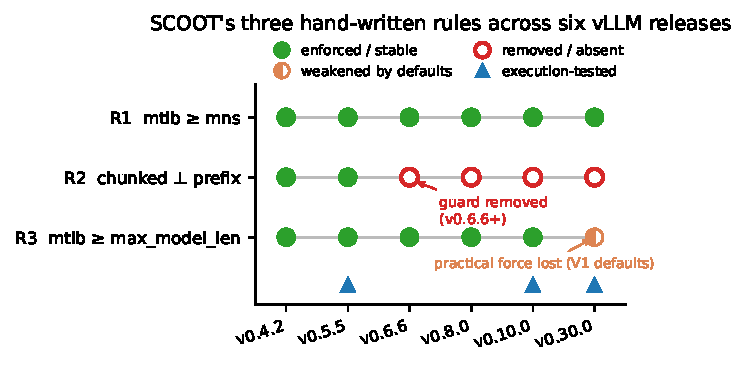
\includegraphics[width=0.98\columnwidth]{fig_drift_rules.pdf}
\caption{The lifecycle of SCOOT's three published rules across six vLLM releases, re-checked at source and (on the marked versions) at execution level. Hand-written constraint knowledge decays: one rule was removed upstream, one survives only nominally.}
\label{fig:drift}
\end{figure}

On llama.cpp v0.5.0 we executed 17 test cases covering seven candidate rules: two real constraints were confirmed (\code{n\_batch >= 1} aborts with SIGABRT when violated; quantized KV cache requires flash attention), while six assumed rules were not enforced, including \code{n\_ubatch <= n\_batch}.

\textbf{Takeaway.} Constraints must be \emph{mined from source} and \emph{verified by execution}, and re-mined as engines evolve.

%% ===========================================================================
\section{Method: Extract--Falsify--Inject}
%% ===========================================================================

\begin{figure*}[t]
\centering
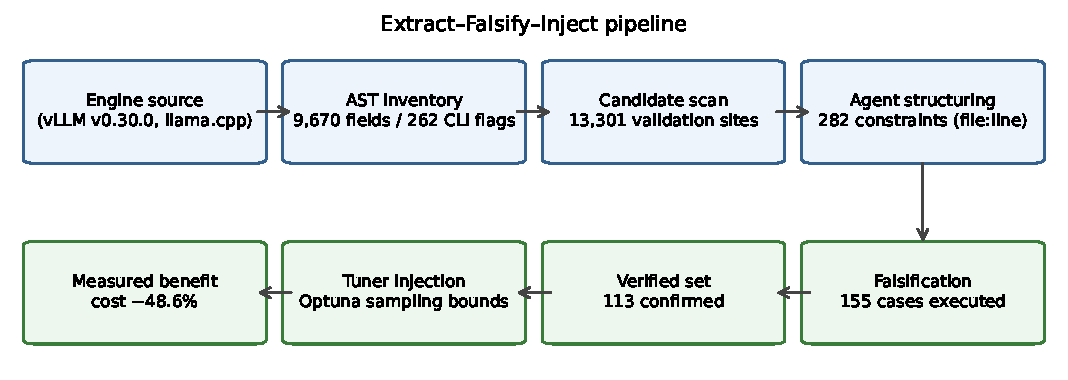
\includegraphics[width=0.92\textwidth]{fig1_pipeline.pdf}
\caption{The extract--falsify--inject pipeline with measured numbers at each stage (9{,}670 fields $\rightarrow$ 13{,}301 validation sites $\rightarrow$ 282 constraints in the core tiers, 716 with the full-coverage extension $\rightarrow$ 155 executed cases $\rightarrow$ 113 confirmed $\rightarrow$ tuning cost $-48.6\%$).}
\label{fig:pipeline}
\end{figure*}

\subsection{Problem formulation}

Let $P = \{p_1, \ldots, p_n\}$ be the engine's configuration parameters with domains $D_i$ (integer/real ranges, enumerations, booleans, structured fields); the \emph{configuration space} is $\Lambda = \prod_i D_i$ and an assignment $\sigma \in \Lambda$ is one launch configuration. A \emph{constraint} is $c = (id, t, \varphi, \pi)$---a type $t$, a predicate $\varphi$ over a parameter subset $\pi \subseteq P$, and provenance. Seven types cover the engines we study: \textbf{inequality} ($x \geq y$), \textbf{range} ($x \in [l,u]$), \textbf{enum} ($x \in S$), \textbf{arithmetic} ($x \bmod y = 0$, $x = c\cdot y$), \textbf{implication} ($A \Rightarrow B$), \textbf{mutual exclusion} ($\neg(A \wedge B)$), and \textbf{structural type}. An assignment \emph{satisfies} $c$ ($\sigma \models c$) iff $\varphi$ evaluates true under $\sigma$; the \emph{legal domain} of a constraint set $C$ is $\Lambda_C = \{\sigma \in \Lambda : \forall c \in C,\ \sigma \models c\}$ and the \emph{nominal pruning ratio} is $\rho_{\text{grid}} = 1 - |\Lambda_C|/|\Lambda|$. A \emph{constraint graph} is $G = (P, C)$ with evidence and validation status per node. Our goal is to produce $G$ with evidence, falsify it by execution, and measure the effect of sampling from $\Lambda_C$ rather than $\Lambda$.

\subsection{Parameter inventory (static)}

We parse the engine tree with Python's AST and extract every class-level annotated assignment (name, type, default, \code{Field} metadata), plus every CLI flag registered via \code{add\_argument}. Each entry stores \code{file}, \code{line}, and the source snippet. For vLLM v0.30.0 this yields 9{,}670 fields and 262 flags; for downstream filtering we keep the \code{vllm/config/} and \code{EngineArgs} subsets (585 $+$ 242).

\subsection{Candidate generation (static)}

We scan for validation sites of two syntactic forms: \code{assert <cond>} and \code{if <cond>: raise \ldots}. On vLLM v0.30.0 this produces \textbf{13{,}301 candidates} (8{,}498 assertions; 4{,}803 guarded raises). We tier candidates by path (\code{vllm/config/} $>$ \code{engine/core} $>$ rest) and keep those whose condition or message mentions at least one parameter name from the inventory, reducing the agent workload to \textbf{3{,}129 candidates} (363 in the two high-priority tiers).

\subsection{Agent-based structuring}
\label{sec:agent}

We partition the high-priority candidates by module and assign one LLM sub-agent per partition (deepseek-v4.1-flash; five partitions, 50--94 candidates each). Each agent re-reads the source around every candidate ($\pm$30 lines) and emits constraints in a fixed schema: \code{type}, \code{expr} over real field names, \code{params}, \code{severity}, a one-sentence \code{mechanism}, and \code{evidence[]} with verbatim snippets. Candidates that are internal invariants, hardware checks, or non-parameter state are dropped with a recorded reason.

A merge stage applies four mechanical checks: (R1) every parameter exists in the inventory; (R2) every evidence line exists; (R3) every snippet appears verbatim on its line; (R4) the expression is non-empty and references declared parameters. Violations are rejected, not silently dropped. \textbf{Result: 282 constraints across 26 scopes, 100\% with evidence, zero mechanical rejections} (after fixing one CLI-destination derivation bug that had initially mis-rejected two legitimate constraints).

\textbf{Cross-model replication.} Re-running the identical pipeline on a second LLM (GLM-5.3-Flash, vs.\ deepseek-v4.1-flash for the primary run; same inputs, schema, and rules) yields 320 constraints. Under the strict evidence-anchor criterion (shared \code{file:line}), \textbf{97.2\% of the primary run's 282 constraints are independently re-discovered}; conversely, 88.1\% of the second run's constraints are covered by the first, and the second run contributes 34 additional candidates (21 error-level). Single-model extraction still has blind spots (8 constraints found only by the primary run), which motivates releasing the union as the artifact.

\subsection{Falsification by execution}

For each constraint we construct a \emph{violating assignment}---falsification by construction, in the spirit of property-based testing~\cite{quickcheck}. Four LLM sub-agents translate constraints into concrete field assignments (e.g., \code{kv\_connector is not None -> kv\_role is not None} becomes \code{\{"kv\_connector": "NixlConnector", "kv\_role": null\}}), skipping constraints whose checks occur at request time or in runtime components. The executor then instantiates the engine's real configuration classes with a \textbf{baseline-first protocol}: a legal baseline must construct successfully, after which the violating override is applied; a constraint is \emph{confirmed} only if the override triggers an error. This guards against counting unrelated construction failures as evidence.

vLLM v0.30.0 specifics (documented for reproducibility): configurations are pydantic models whose \code{dataclasses.fields} expose \code{FieldInfo} defaults; \code{SchedulerConfig} requires ``virtual'' keys (\code{max\_model\_len}, \code{is\_encoder\_decoder}) consumed by a before-validator; nested configs must be built as sub-objects; \code{ModelConfig} can be constructed offline from a local tiny model. We validate 155 constraints this way (\S\ref{sec:rq2}). For llama.cpp we execute the real CLI binary and capture exit codes and stderr.

\textbf{Witness-level confirmation (Proposition~1).} If the protocol confirms $c$ on version $V$, then $V$'s validation path rejected the constructed violating witness. If the validator is \emph{total} over $\pi$ (it rejects \emph{every} violating assignment, not a subset), confirmation extends to all protocol-reachable assignments sharing the tested code path. We state this as a proposition, not a universal guarantee: a validator may guard only some branches---our adversarial audit found three branch-precondition omissions among 30 nodes---and the evidence covers only (i) protocol-reachable construction paths, since cross-configuration and runtime constraints remain \code{not-tested} (\S\ref{sec:rq2}), and (ii) the tested version, since constraint knowledge drifts (\S\ref{sec:rq3}). Every graph node therefore carries a version and a validation status.

\subsection{Injection into the tuner}
\label{sec:inject}

\textbf{Generic constrained sampler.} We inject $C$ as \emph{derived sampling domains} rather than hard-coded bounds. For a parameter $x$ and an already-sampled assignment $\sigma'$, the reachable domain is $R(x \mid \sigma', C) = D_x \cap \bigcap_{c\ \text{evaluable}} \text{bound}_c(x, \sigma')$, where $\text{bound}_c$ raises or lowers integer bounds ($x \geq y \Rightarrow \text{lo}(x) \leftarrow \max(\text{lo}(x), y)$; $x \geq c\cdot y$; $x < y \Rightarrow \text{hi}(x) \leftarrow y-1$), restricts to multiples ($x \bmod y = 0$), or filters enumerations. The sampler walks parameters in dependency order and samples within $R$. The implementation reads the graph JSON directly---a data-driven injection, demonstrated on a six-dimensional space in \S\ref{sec:rq5}.

\textbf{Zero-violation sampling (Proposition~2).} The sampler never returns a violating assignment: at each step it samples inside the intersection of all currently evaluable bounds, and reports failure (no sample) when that intersection is empty. It \emph{succeeds} whenever every step's feasible domain is non-empty---an assumption, not a guarantee: the 716-node graph contains 7 cyclic implication clusters (largest cycle 3), for which no linear dependency order exists and bounds are instead computed from constraint evaluability as parameters are assigned. No empty-domain failure occurred in the 90 sampler-in-loop runs (\S\ref{sec:rq5}).

\textbf{From coverage to cost.} With $n$ trials, violation rate $r$, and invalid-trial cost $c_{\text{inv}}$, the expected cost is $n(1 + c_{\text{inv}} r)$, so constraining $r_b \rightarrow r_a$ saves $c_{\text{inv}}(r_b - r_a)/(1 + c_{\text{inv}} r_b)$; the saving exceeds 30\% iff $r_b \geq 3/(7 c_{\text{inv}})$ (e.g., $r_b \geq 14.3\%$ at $c_{\text{inv}} = 3$). Crucially, $r$ must be computed under the \emph{tuner's sampling distribution}: the nominal grid ratio (${\approx}12\%$ in our two-dimensional space) badly underestimates the waste of log-uniform sampling (83.3\% for the six-dimensional space, analytically 66.7\% from the token-budget constraint and ${\approx}50\%$ from the KV-capacity rule); an adaptive sampler (TPE~\cite{tpe}, via Optuna~\cite{ref7}) partially mitigates it (31.5\% measured), and constraint injection removes it entirely (0\%) (Figure~\ref{fig:sampler}). \S\ref{sec:rq5} verifies the analytical saving (48.6\%) against the measured value.

%% ===========================================================================
\section{Evaluation}
%% ===========================================================================

\subsection{Setup}
\label{sec:setup}

\begin{table}[t]
\centering
\caption{Experimental setup.}
\label{tab:setup}
\small
\begin{tabular}{@{}>{\raggedright\arraybackslash}p{2.3cm}>{\raggedright\arraybackslash}p{5.1cm}@{}}
\toprule
Component & Details \\
\midrule
Engines & vLLM v0.30.0 (commit \code{ced6857}; configuration-construction validation, no GPU); llama.cpp 0.5.0-dev build 11194 (real execution, CPU); Vidur~\cite{ref6} (MLSys'24 simulator, vLLM-V0 semantics) for tuning \\
Hardware & One laptop: Intel i5-7300HQ (4 cores), 23.7\,GB RAM; the installed GTX 1050 (CC 6.1) is unsupported by vLLM, so all experiments are CPU-only. Cash cost: \textyen 0 \\
Model (anchor) & Qwen2.5-0.5B-Instruct (anchor grid) and Qwen2.5-1.5B-Instruct (micro-study), Q4\_K\_M, for llama.cpp \\
Tuning spaces & S5: 2-D/5-D (\code{mns} $\times$ \code{mtib} $\times$ \code{block\_size} $\times$ \code{watermark}; \code{block\_size} fixed to 16 by the simulator). Dimension scaling adds explicit \code{num\_blocks} (\textbf{6-D}, with the KV-capacity rule) and workloads at qps $\in \{8,12,16\}$ \\
Reproducibility & Every artifact records engine commit, configuration, metrics, and cost; scripts and raw records released (\S\ref{app:artifact}) \\
\bottomrule
\end{tabular}
\end{table}

\subsection{RQ1: How good is the extraction?}
\label{sec:rq1}

\textbf{Static layer}: 9{,}670 annotated fields; 262 CLI flags; 13{,}301 validation candidates; 3{,}129 parameter-related; 363 in high-priority tiers.

\textbf{Agent layer}: 282 constraints from the configuration/engine tiers (implication 127, mutual exclusion 42, range 33, arithmetic 26, enum 24, inequality 22, type 8; Figure~\ref{fig:types} shows both tiers; top scopes \code{vllm\_config} 61, \code{speculative} 36, \code{parallel} 27). Extending coverage to all 3{,}129 parameter-related candidates (10 additional agent batches over the remaining 2{,}766 sites) adds 434 more constraints, for \textbf{716 total}, all with verbatim source evidence.

\begin{figure}[t]
\centering
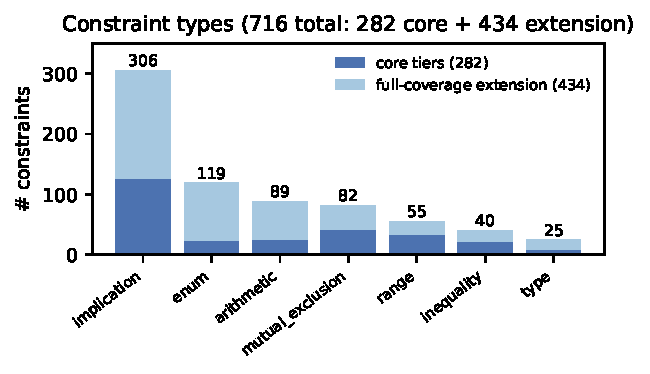
\includegraphics[width=0.95\columnwidth]{fig2_types.pdf}
\caption{Constraint type distribution: core tiers (282) and full-coverage extension (434), by type.}
\label{fig:types}
\end{figure}

\textbf{Audits.} A seeded random sample of 20 constraints was checked against source line-by-line by the pipeline operator: \textbf{16 fully correct, 4 partially precise, 0 incorrect}. An independent second batch (different seed; reviewer role) scored \textbf{20/20 correct}. Across both batches (40 constraints, two independent samples), \textbf{no constraint was found incorrect}. A further \textbf{adversarial} audit (30 constraints; a fresh instance explicitly instructed to refute them) also found \textbf{0 incorrect}; its three partial findings are branch-precondition omissions, now recorded as \code{audit\_note}s in the released graph. Cumulative: \textbf{130 constraint-audits, 0 incorrect}. All audits in this paper were produced by pipeline roles or independent AI instances; for the 150-site labeling kit, an independent human labeler (a technically literate non-expert following the released instructions) has since repeated the pass: agreement with the evaluator labels is 75.3\% raw / $\kappa=0.53$ and with the third pass 83.9\% / $\kappa=0.68$---comparable to the AI-vs-AI agreement---and the human labels reproduce the capture estimate (84.8\% equal-weight and 72.2\% constraint-weighted $\pm$1 line); the human is again stricter than the evaluator, the same direction as every independent pass.

\textbf{Recall (gold standard).} Two independent stratified samples (300 sites total; 50 per tier per sample, fixed seeds; population tier sizes 244/119/2{,}766) were labeled against source by the evaluator: 203 true constraints and 97 non-constraints. Under \emph{equal weighting across tiers}, the pipeline captures \textbf{71.9\%} of the true constraints by exact evidence line and \textbf{87.2\% within $\pm$1 line} (Wilson 95\% CI [65.4, 77.7] and [81.9, 91.1]); because tier-3 sites dominate the population (88.4\%), the site-level \emph{design-weighted} estimates (weights = candidate count per tier, 244/119/2{,}766) are \textbf{50.8\% (exact) and 59.5\% ($\pm$1)} (95\% CI $\approx$ [42.1, 59.5] and [50.9, 68.1]); weighting instead by the estimated number of true constraints per tier (the estimand for ``recall over all true constraints'') gives \textbf{53.0\% (exact) and 63.2\% ($\pm$1)}---we report all three estimands and quote the equal-weight one in the abstract. The intervals treat the stratified samples as simple random; with tier~3 dominating the population they are approximate. By tier (exact/$\pm$1): 66\%/96\% (config), 94\%/96\% (engine/core), 48\%/55\% (model/kernel); 5 of 97 non-constraint sites carry graph evidence. Recall is line-level (does the graph anchor the labeled site?); expression-level correctness is audited separately above. An independent blind labeling pass (a different model instance; 120 audited sites; identical criteria) agrees at 80.0\% raw / $\kappa = 0.60$ (per batch 0.75 and 0.46); 23 of 24 disagreements are in the direction of the evaluator being more inclusive, and they span internal-invariant \emph{and} configuration-layer checks. On the batch-2 60-site subset, $\pm$1-line recall is 79.1\% under evaluator labels and \textbf{92.3\%} under the stricter independent labels, so the sensitivity concentrates in the disputed sites. A third independent pass over 150 of the same sites---executed blind through the released labeling kit (site material only; no capture information; fresh-context instances)---agrees with the evaluator labels at \textbf{82.6\% raw / $\kappa=0.65$} and yields \textbf{88.3\% equal-weight and 75.3\% design-weighted $\pm$1-line capture} under its stricter labels (exact: 66.7\%/48.4\%).

\textbf{An independent, non-scanner frame.} To test whether this estimate is an artifact of the candidate funnel, we drew a separate frame without using any scanner output: 150 of the 2{,}479 files in \code{vllm/} (fixed seed), with every \code{assert}/\code{raise} site enumerated by an independent AST pass; a name table of engine-configuration fields pre-filtered the 98 strongest candidates, which were then adjudicated one by one by a single adjudicator (the pipeline operator). Fifty are engine-configuration validation sites, of which the released graph captures \textbf{34 by $\pm$1 line (68.0\%, Wilson 95\% CI [54.2, 79.2]; 24 exact-line)}---a lower estimate than the candidate-pool frame under the same $\pm$1 criterion (87.2\%, CI [81.9, 91.1]; the intervals do not overlap), which we read as a \emph{scope} difference rather than a corroboration: the independent frame samples the whole source tree, the funnel frame the scanner's candidates; the 16 residuals sit in attention-backend quantization/dtype combinations, per-model TP divisibility checks, and runtime-state modules (\code{forward\_context}, \code{hisparse}) outside the tier plan. The frame also shows that most \code{assert}/\code{raise} sites in the tree are not configuration constraints at all (kernel, tensor, and checkpoint checks)---the engine-configuration surface is a small, identifiable slice, and \S\ref{sec:limitations} states its boundaries explicitly.

\textbf{Cross-model robustness} (\S\ref{sec:agent}): 97.2\% evidence-anchored re-discovery by an independent LLM run.

\subsection{RQ2: Do the constraints hold in the real engine?}
\label{sec:rq2}

155 constraints were constructible; 127 (45\%) were classified as runtime/request-time/environmental and not constructible offline---this is the construction-path protocol's boundary, not a correctness claim (SCOOT's rule~\#2 is exactly such a runtime guard, \S\ref{sec:drift}).

\begin{table}[t]
\centering
\caption{Falsification outcomes (vLLM v0.30.0, 155 executed cases).}
\label{tab:falsify}
\small
\begin{tabular}{@{}>{\raggedright\arraybackslash}p{2.0cm}>{\raggedright\arraybackslash}p{2.6cm}>{\raggedright\arraybackslash}p{2.9cm}@{}}
\toprule
Status & Count & Meaning \\
\midrule
\textbf{confirmed (primary)} & \textbf{111} & violating assignment triggers a real engine error \\
confirmed (cross-model) & 2 & same protocol, second LLM batch \\
no\_error & 22 & baseline constructs; violation not triggered at construction \\
blocked & 22 & construction dependencies (heavy configs) \\
\midrule
total executed & 157 & 155 constructible primary cases $+$ 2 cross-model cases \\
\bottomrule
\end{tabular}
\end{table}

Confirmed constraints include the flagship rule mined automatically from source: \code{mtib >= mns} $\rightarrow$ \code{ValueError: max\_num\_batched\_tokens (16) must be greater than or equal to max\_num\_seqs (32)} (\code{vllm/config/scheduler.py:309}), plus 23 parallel-topology rules, 16 speculative-decoding~\cite{ref13} rules, 10 profiler rules, and 8 compilation rules (Figure~\ref{fig:typestatus}).

\begin{figure}[t]
\centering
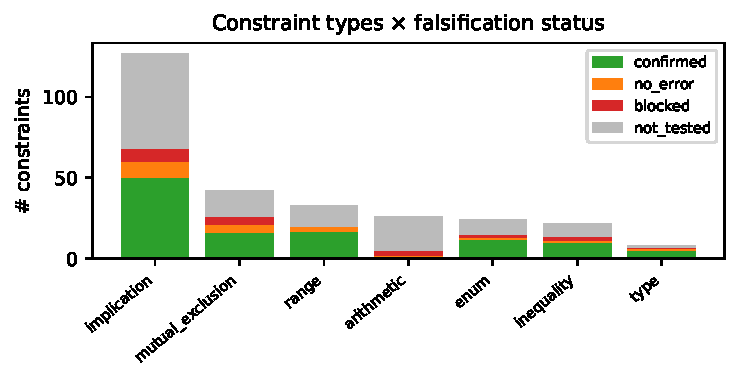
\includegraphics[width=0.95\columnwidth]{fig7_type_status.pdf}
\caption{Confirmation status by constraint type.}
\label{fig:typestatus}
\end{figure}

\begin{figure}[t]
\centering
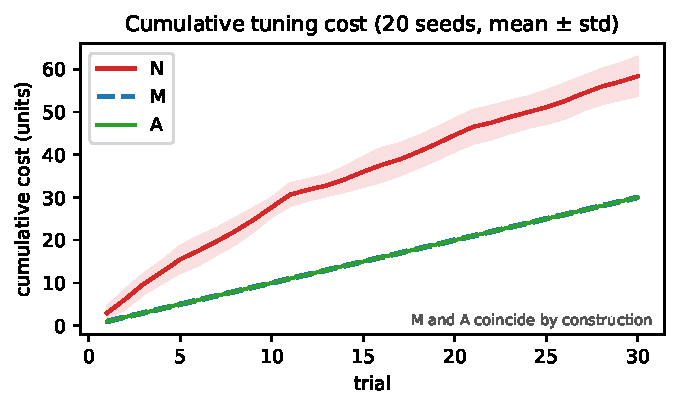
\includegraphics[width=0.95\columnwidth]{fig3_cost_curves.pdf}
\caption{Cumulative tuning cost (S5 three-arm study, 20 seeds).}
\label{fig:cost}
\end{figure}

\subsection{RQ3: Do hand-written constraints survive version drift?}
\label{sec:rq3}

No---see \S\ref{sec:drift}. Of SCOOT's three rules: \textbf{one is stable across five releases} (execution-confirmed on v0.5.5, v0.10.0, and v0.30.0); \textbf{one was a runtime-enforced constraint in the anchor versions that upstream later removed} when it added support for the combination (v0.4.2/v0.5.5 \code{worker/model\_runner.py} raises on a prefix-cache hit under chunked prefill; the guard is absent from the main runner in v0.6.6 onward---and construction-path checks never rejected the combination, which is why our construction tests at v0.5.5/v0.10.0/v0.30.0 all pass); \textbf{one keeps identical semantics but lost practical force} because V1 enables chunked prefill~\cite{ref14} by default. On llama.cpp, 2 of 17 executed configurations confirmed real constraints and 6 assumed rules were not enforced. \textbf{Hand-written constraint sets decay; and runtime guards sit outside construction-path verification---automatic extraction with execution verification is necessary.}

\subsection{RQ4: Does the protocol transfer across engines?}

The same extraction protocol applied to \textbf{SGLang v0.5.20} (a different configuration architecture: \code{ServerArgs} validation hooks) yields \textbf{420 constraints} with 100\% source evidence and zero mechanical rejections; the constraint-family profile mirrors vLLM's---KV-cache/memory, parallelism/topology, quantization, and speculative decoding dominate. A quality audit on a type-stratified sample of 40 constraints (plus a blind re-audit of 20 by an independent pass) found \textbf{0 incorrect constraints} (60 constraint-audits); the single disagreement---a path exception not recorded in the expression---was fixed in the released graph.

The falsification protocol applied to llama.cpp (a C++ engine) confirmed two constraints and refuted six (\S\ref{sec:drift}). Real measurements over 24 configurations (threads $\in \{2,3,4\}$ $\times$ batch $\in \{128,256,512\}$ $\times$ ubatch $\in \{64,128,256\}$; 5 repetitions each) show prompt-processing up to \textbf{159.8\,tok/s} and generation up to \textbf{45.9\,tok/s} on the 0.5B model---establishing that the method is not vLLM-specific and that our records capture real, not simulated, behavior.

\subsection{RQ5: What is the tuning benefit?}
\label{sec:rq5}

\textbf{Setup.} Vidur~\cite{ref6} (vLLM-V0 semantics), LLaMA-2-7B on A100, trace \code{splitwise\_conv}~\cite{splitwise} (19{,}366 requests), 384 requests per run, Poisson arrivals at qps${}=12.0$. We calibrated the workload first: the system's capacity is ${\approx}9.4$\,rps; at qps${}=8$ the objective is arrival-limited and non-discriminative, whereas at qps${}=12$ representative configurations span goodput \textbf{0.79--8.96}. SLO: TTFT-p90 $\leq$ 1.0\,s and TPOT-p90 $\leq$ 0.1\,s. Search space: \code{max\_num\_seqs} $\in [16,256]$ (log) $\times$ \code{max\_num\_batched\_tokens} $\in [16$ or $\max(\text{seqs},1024), 8192]$ (log) $\times$ \code{watermark} $\in [0.001,0.2]$ (log); \code{block\_size} is fixed to 16 because the simulator's bundled profiling data only supports 16 (a simulator limitation, not a real-engine constraint).

\textbf{Arms.} \textbf{N} no constraints; \textbf{M} manual (SCOOT-projected: \code{mtib} $\geq \max(\text{mns}, 1024)$, i.e., rule~\#1 plus the no-chunked-prefill rule~\#3 in V0 semantics); \textbf{A} automatic (mined graph projected); \textbf{S} SCOOT-style (only the manual rule, with online boundary learning from failures). Each arm: 20 seeds $\times$ 30 trials $=$ 600 trials; 1{,}800 simulations in 238 minutes.

\begin{table}[t]
\centering
\caption{Headline three-arm study (20 seeds $\times$ 30 trials per arm).}
\label{tab:headline}
\footnotesize
\setlength{\tabcolsep}{4pt}
\begin{tabular}{@{}lcccc@{}}
\toprule
Arm & Cost (units) & Invalid rate & Best goodput & Trials-to-target \\
\midrule
N & 58.350 $\pm$ 4.614 & 31.5\% $\pm$ 5.1\% & 8.954 $\pm$ 0.027 & 9.80 $\pm$ 5.57 \\
M & 30.000 $\pm$ 0.000 & 0\% & 8.987 $\pm$ 0.029 & 5.35 $\pm$ 2.66 \\
A & 30.000 $\pm$ 0.000 & 0\% & 8.987 $\pm$ 0.029 & 5.35 $\pm$ 2.66 \\
\bottomrule
\end{tabular}
\end{table}

\textbf{Findings.} Cost \textbf{$-48.6\%$} by ratio of means (paired per-seed reduction 48.3\%, 95\% CI [46.7\%, 50.0\%]); trials-to-target $-45.4\%$ (N: 9.80 [7.45, 12.25] vs.\ M/A: 5.35 [4.15, 6.45]; target $=0.9\times$ the pooled best goodput, defined here for the first time---no censoring occurs, max 21/30); charged invalid sampling 31.5\% $\rightarrow$ 0\%; final quality not reduced (8.954 $\rightarrow$ 8.987, paired difference $+0.033$). We designate the S5 N$\rightarrow$M cost reduction as the single primary endpoint; all cross-space/cross-load numbers are exploratory. Cost sensitivity to the illegal-trial penalty: reductions of 24.0\% / 48.6\% / 75.9\% at $c_{\text{inv}} = 1/3/10$.

\textbf{Two honest notes.} (i)~In the simulator's small parameter subspace, arms M and A are \emph{equivalent by construction}: the projected constraint is the same single bound, and \textbf{the effective constraint in this subspace is a single load-derived lower bound} (\code{mtib} $\geq 1024$, the trace's practical prefill threshold)---RQ5 therefore quantifies the value of \emph{having} that bound, while the value of \emph{automatic} extraction is established by RQ1--RQ4, not by RQ5. (ii)~The constraint's \emph{discrete} space reduction is only 12.3\% (1.97M $\rightarrow$ 1.73M grid points), yet it removes about two-thirds of log-uniformly drawn samples before the optimizer adapts (31.5\% charged-invalid): the value of a constraint depends on the sampler's distribution, so both figures are reported. Figures~\ref{fig:cost}--\ref{fig:box} show cumulative cost, best-so-far goodput, and per-seed cost distributions.

\begin{figure}[t]
\centering
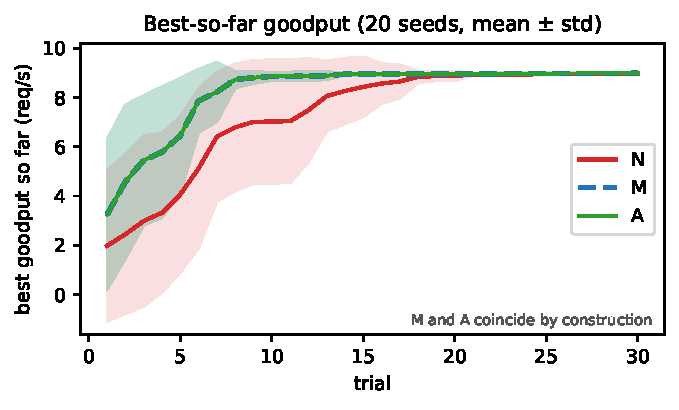
\includegraphics[width=0.95\columnwidth]{fig4_convergence.pdf}
\caption{Best-so-far goodput (S5).}
\label{fig:conv}
\end{figure}

\begin{figure}[t]
\centering
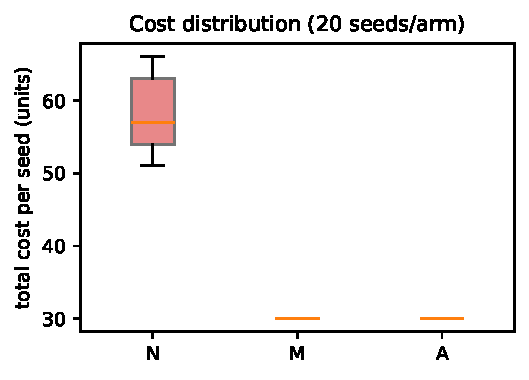
\includegraphics[width=0.95\columnwidth]{fig5_cost_box.pdf}
\caption{Per-seed cost distributions (S5).}
\label{fig:box}
\end{figure}

\textbf{Data-driven injection in the loop (six dimensions).} We validate the generic sampler of \S\ref{sec:inject} end-to-end: the constraint graph JSON (716 nodes plus two auxiliary rules---one execution-discovered load bound and one simulator-derived KV-capacity rule, which is a performance/capacity rule rather than a legality constraint) is read directly and drives sampling in a six-dimensional space. Across 3 seeds $\times$ 30 trials $=$ \textbf{90 real simulations, constraint violations and run failures are both 0/90, and cumulative cost equals the theoretical minimum (30.0 units)}; best goodput matches the hard-coded arm. This closes the loop from ``constraint graph JSON'' to tuner behaviour with no hand-written bounds.

\textbf{Dimension scaling and workload robustness.} Two further studies quantify how the benefit depends on the space and the load (same cost model; seeds 1--10; the 5-D row reuses the S5 runs).

\begin{table}[t]
\centering
\caption{Dimension scaling (qps${}=12$, seeds 1--10); the 6-D space adds an explicit \code{num\_blocks} dimension.}
\label{tab:dimension}
\footnotesize
\setlength{\tabcolsep}{4pt}
\begin{tabular}{@{}lcccc@{}}
\toprule
Space & N cost & M/A cost & N$\to$M/A reduction & N invalid \\
\midrule
2-D & 61.20 $\pm$ 2.90 & 30.00 $\pm$ 0.00 & \textbf{50.9\% [49.3, 52.1]} & 35\% \\
5-D (S5) & 58.80 $\pm$ 5.33 & 30.00 $\pm$ 0.00 & \textbf{48.6\% [45.9, 51.3]} & 32\% \\
6-D & 53.40 $\pm$ 4.43 & 30.00 $\pm$ 0.00 & \textbf{43.5\% [40.9, 46.2]} & 26\% \\
\bottomrule
\end{tabular}
\end{table}

The constrained arms stay at the theoretical minimum (30.0 units) in every space, while the unconstrained arm's cost \emph{falls} as dimensions grow (61.2 $\rightarrow$ 58.8 $\rightarrow$ 53.4 units): with more knobs the optimizer partially routes around violations, so the \emph{relative} benefit is largest in small spaces but remains ${>}40\%$ even at 6-D. In the 6-D space the N arm violates the KV-capacity rule in \textbf{41.3\%} of trials (124/300) versus 0\% for the constrained arms. Workload robustness (5-D, qps $\in \{8,12,16\}$) gives reductions of \textbf{48.3\%, 48.6\%, and 49.6\%}---stable across load regimes (Figure~\ref{fig:dimcurve}).

\begin{figure}[t]
\centering
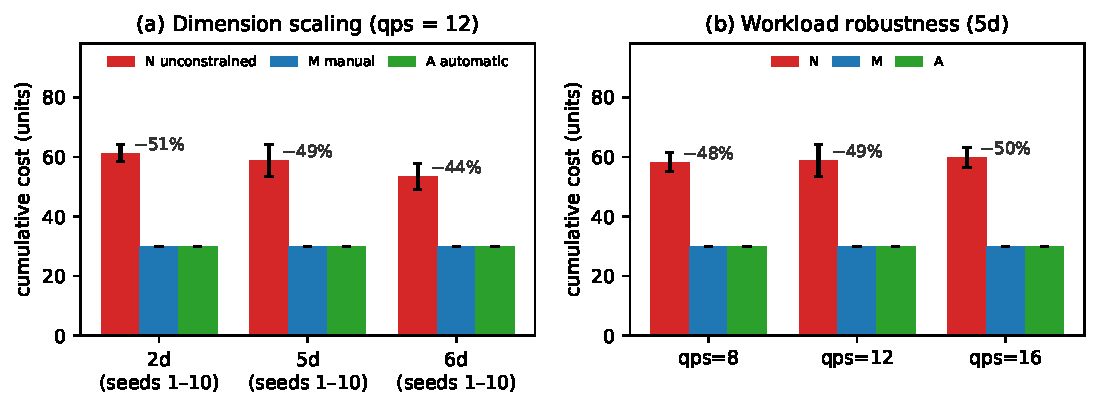
\includegraphics[width=0.98\columnwidth]{fig8_dimension_curve.pdf}
\caption{Dimension scaling and workload robustness.}
\label{fig:dimcurve}
\end{figure}

\textbf{SCOOT-style online learning vs.\ automatic extraction.} To isolate the value of \emph{automatic} extraction from \emph{online} learning, the \textbf{S arm} emulates SCOOT's mechanism: only the manual rule \code{mtib} $\geq$ \code{mns} is enforced, and the lower bound is raised online whenever a trial fails (monotone boundary learning). Over 20 seeds, S costs \textbf{38.55 $\pm$ 2.80 units} (invalid rate 9.5\%)---better than N ($-33.5\%$) but \textbf{21.8\% worse than the source-mined arms} (paired CI [19.3, 24.2]): online learning recovers most of the constraint surface, but it pays for the rediscovery in invalid trials, whereas extraction from source eliminates them from trial 1.

\textbf{Real-engine A$\neq$M micro-study (llama.cpp).} RQ5's main arms share the simulator's constraint vocabulary; to test the distinction on a real engine against \emph{folklore} rather than projected rules, we tuned llama.cpp v0.5.0 (Qwen2.5-1.5B-Instruct, four-core CPU) over six dimensions---threads, \code{n\_batch}, \code{n\_ubatch}, flash attention, and K/V cache types (216 combinations; objective pp256). Four arms run 5 seeds $\times$ 20 trials each, interleaved trial-by-trial with a fixed calibration configuration to cancel the machine's thermal drift: \textbf{N} no constraints; \textbf{M} the folk rule \code{n\_ubatch}$\leq$\code{n\_batch} (refuted by our execution tests, \S\ref{sec:rq2}); \textbf{A} the source-mined, execution-confirmed constraint (quantized V-cache $\Rightarrow$ \code{flash\_attn}; \code{n\_batch}$\geq$1 is non-binding in this space); and \textbf{S} a SCOOT-style arm that starts from M's folk rule and \emph{learns from failures}---after the first violating trial it forces attention on whenever V-cache quantization is sampled. \textbf{A incurs 0 of 100 invalid trials}; \textbf{S pays exactly one discovery failure per seed (5\% total) before its learned rule takes over}; \textbf{M and N pay 12 and 17}---all 34 failures being precisely \code{ctv=q8\_0} with \code{fa=off}, the combination A forbids. \textbf{M and S never sample the legal \code{ubatch}$>$\code{batch} region (0/88 and 0/95 vs 11/100 for A and 14/83 for N)}, which the engine accepts. Cumulative cost (success 1, failure 4 units): \textbf{A 20.0 $\pm$ 0.0 $<$ S 23.0 $\pm$ 0.0 $<$ M 27.2 $\pm$ 4.0 $<$ N 30.2 $\pm$ 1.6}; paired gaps to A: \textbf{$-13.0\%$ (S, 95\% CI [3.0, 3.0] units), $-26.5\%$ (M, [2.2, 12.2]), $-33.8\%$ (N, [8.2, 12.2])}. The folk rule is simultaneously \emph{incomplete} (it misses the constraint that fails) and \emph{over-restrictive} (it forbids legal configurations); online learning recovers after one paid failure per study---the price of rediscovering what the source already states---whereas only source mining eliminates invalid trials from trial 1. \emph{Final quality.} Re-running each arm's best configuration with three repeats (rotated within seeds) shows no separation in attainable throughput---per-arm medians 48.5--63.3\,t/s with fully overlapping ranges---on this machine the environment, not the arm, dominates absolute numbers; constraints change the \emph{cost} of the search, not the peak it reaches.

\textbf{Workload transfer.} Repeating the full protocol on two workloads with far longer prefills---summarization (\code{arxiv}, prefill p50 ${\approx}2.7$K) and code (\code{splitwise\_code}, p90 ${\approx}5.2$K)---gives N$\rightarrow$M/A reductions of \textbf{46.2\% [43.6, 48.7]} and \textbf{48.3\% [46.9, 49.8]}, with the constrained arms again at the theoretical minimum and the online-learning penalty stable at 23.1\% and 20.3\%. Notably, the load constraint's empirical threshold is \textbf{trace-independent}: on all three traces, failures occur at \code{mtib} $\leq 1008$ and the smallest successful value is $\geq 1025$---a correctly mined constraint transfers across workloads without re-calibration.

\begin{figure}[t]
\centering
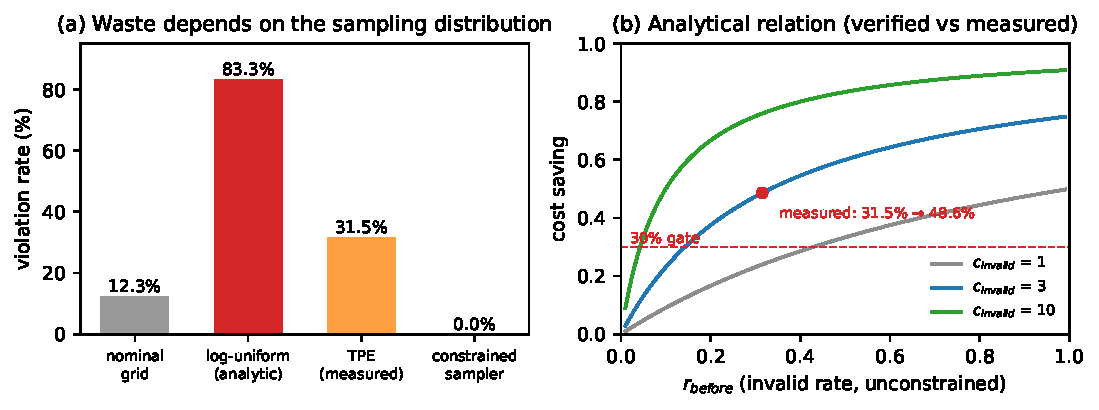
\includegraphics[width=0.98\columnwidth]{fig9_sampler_analysis.pdf}
\caption{Why the violation rate depends on the sampling distribution (left) and the analytical saving relation verified against the measured value (right).}
\label{fig:sampler}
\end{figure}

\subsection{Cost accounting}

\begin{table}[t]
\centering
\caption{Cost accounting.}
\label{tab:cost}
\small
\begin{tabular}{@{}>{\raggedright\arraybackslash}p{2.4cm}>{\raggedright\arraybackslash}p{5.0cm}@{}}
\toprule
Item & Value \\
\midrule
GPU hours & 0 (vLLM validation is CPU; tuning is simulation; anchor is CPU llama.cpp) \\
Wall clock & extraction ${\approx}$hours (agent time); falsification ${\approx}$minutes; tuning ${\approx}$238\,min (S5) $+$ ${\approx}$5\,h (dimension/workload) $+$ 25\,min (sampler) $+$ ${\approx}$1.5\,h (request-length workloads) \\
Cash & \textyen 0 \\
Simulation scale & \textbf{8{,}000+ simulated trials} (301 Optuna studies across arms/spaces/loads; real-hardware studies typically afford tens) \\
\bottomrule
\end{tabular}
\end{table}

%% ===========================================================================
\section{Related Work}
%% ===========================================================================

\textbf{Inference engine tuning.} SCOOT~\cite{ref2} is the closest system: Bayesian optimization with hand-written known constraints and online-learned hidden constraints. We emulate its mechanism explicitly: its known-constraint component corresponds to our M arm and its online learning to our S arm. Across 20 seeds, the SCOOT-style arm costs 38.55 $\pm$ 2.80 units (9.5\% invalid) versus 30.00 $\pm$ 0.00 for source-mined constraints---a \textbf{21.8\% [19.3, 24.2] gap} representing the price of rediscovering, through invalid trials, constraints already stated in the source; and because two of SCOOT's three published rules have since decayed (\S\ref{sec:drift}), its hand-written set does not cover the constraints that matter for this workload. We do not run SCOOT's full implementation (its BO and crash-handling engineering are outside our emulation), so the comparison is mechanism-level. Our work supplies what SCOOT assumes: constraint \emph{provenance} (source), \emph{verification} (execution), and \emph{maintenance} (re-extraction).

\textbf{Configuration analysis and validation.} Nadi et al.~\cite{ref20} pioneered mining configuration constraints from source---C code, via build-time errors and heuristics, for variability models; we revisit the problem with LLM agents and execution falsification for LLM engines. Dynamic invariant detection~\cite{daikon} infers likely invariants from executions rather than from source. cDep~\cite{ref5} statically extracts five types of configuration dependencies from Java/Scala bytecode and explicitly calls for NLP-based discovery of dependencies \emph{between multiple parameters}---a call our LLM-based extraction answers---but its output is dependency facts for developers, not executable pruning rules with execution-based verification. Configuration diagnosis~\cite{ref16} and white-box performance analysis~\cite{ref17} analyze deployed systems rather than mining constraints from source. PerfSense~\cite{ref3} and its journal successor CongSense~\cite{ref4} use LLM agents over call graphs and documentation to \emph{classify} performance-sensitive parameters. Ciri~\cite{ref21} uses LLMs to \emph{validate given configurations} (misconfiguration detection); it consumes configurations, whereas we mine constraints from source and inject them into a tuner. Configuration errors are a long-studied systems problem---surveys and diagnosis~\cite{xuszsurvey,yinsosp13}, production configuration management~\cite{tangsosp15}, specification synthesis~\cite{configv}, and configuration testing~\cite{ctest4j}---but these lines validate, manage, or test \emph{given} configurations rather than mining cross-parameter constraints for tuning. A parallel line infers constraints from logs (ConfInLog~\cite{confinlog}, ICPC'21) and applies configuration-aware static taint analysis for diagnosability (ConfTainter~\cite{conftainter}, ASE'23; ConfLogger, ICSE'26); these target misconfiguration diagnosis, not tuner-facing constraint sets. Finally, Pimp My LLM~\cite{pimpmyllm} treats LLM inference hyperparameters as a configurable system and manages constraints through a hand-built feature-based variability model---the closest neighbor on the inference-configuration side; unlike our pipeline, its constraints are neither mined from source nor verified by execution.

\textbf{Knowledge-enhanced tuning.} GPTuner~\cite{ref9} reads DBMS \emph{manuals} to extract knob dependencies and value ranges for Bayesian optimization; LLMConf~\cite{ref22} uses a knowledge base to select parameters and their value ranges; LaTune~\cite{ref23} adapts tuning to edge devices via knowledge transfer; InferLog~\cite{inferlog} tunes inference-engine configurations for log-parsing workloads. These systems rely on documentation or curated knowledge bases; we mine from \emph{source} with verbatim evidence and verify by execution.

\textbf{LLM agents for science and code.} LLM agents are increasingly applied across software engineering~\cite{llm4sesurvey}. POPPER~\cite{ref8} validates free-form hypotheses via sequential falsification with e-value error control; our falsification targets deterministic code constraints instead of statistical hypotheses.

\textbf{Simulation.} Vidur~\cite{ref6} predicts inference latency with ${<}9\%$ error and ships Vidur-Search, an enumerative configuration search whose space is human-defined; we use Vidur as an oracle and treat its hard-coded space as a contrast case.

\textbf{Classical configuration tuning} in databases, Spark, and compilers (e.g., database knob tuning~\cite{ituned,ottertune,llamatune}, Rover~\cite{ref10}, BaCO~\cite{ref11}, HEBO~\cite{ref12}) shares the Bayesian machinery but not the source-mined constraint problem.

%% ===========================================================================
\section{Limitations and Threats to Validity}
\label{sec:limitations}
%% ===========================================================================

\begin{enumerate}
  \item \textbf{Simulation fidelity.} RQ5 uses a validated simulator (Vidur, ${<}9\%$ error~\cite{ref6}) under vLLM-V0 semantics; V1-specific constraints do not participate. Relative comparisons are the paper's currency; a GPU-based replication is future work.
  \item \textbf{Offline-constructible subset.} 127 of the 282 core-tier constraints are runtime/request-time checks not exercised by construction-path falsification; they are marked, not claimed. Cross-engine real execution partially compensates (llama.cpp).
  \item \textbf{Anchor scale.} The llama.cpp evidence spans a 0.5B anchor grid and a 1.5B four-arm micro-study, both on a four-core CPU; absolute numbers do not represent GPU serving.
  \item \textbf{Simulator artifact.} \code{block\_size} is fixed to 16 because the bundled profiling data only supports 16; this is a simulator limitation, not a real-engine constraint.
  \item \textbf{LLM dependence.} Extraction quality depends on the agent model and prompts---the general risks of LLM-based methods~\cite{ref19}; we mitigate with mechanical evidence checks, independent audits, an evidence-or-drop policy, and cross-model replication (97.2\%).
  \item \textbf{Version coverage.} Execution re-checks cover three versions (v0.5.5, v0.10.0, v0.30.0); systematic execution across all releases remains future work.
  \item \textbf{Evaluator independence.} Audits and gold-standard labels were produced by pipeline roles and independent AI labeling passes rather than by external human experts; across five passes (60+60+30+150 AI sites, plus a 150-site human pass) they agree at $\kappa = 0.46$--$0.79$ (human vs evaluator 0.53; human vs third pass 0.68), 23 of 24 disagreements in the first comparison run in the direction of the evaluator being more inclusive, and the stricter labels raise $\pm$1-line recall to 92.3\% on the batch-2 subset. One independent human labeler has now completed the 150-site kit pass; the full 300-site gold-standard frame and the 130 constraint audits remain AI-labeled, so a human sign-off for the complete release stays on the artifact checklist.
  \item \textbf{Syntax coverage bias.} The headline gold-standard frame is the pipeline's own candidate funnel (\code{assert}/\code{if-raise} sites mentioning an inventory parameter); other enforcement mechanisms (argparse checks, unguarded raises, type/enum annotations, warning-and-fallback branches, and the C++ engines' internals) remain outside both numerator and denominator, so recall is conditional on the scanner's syntactic coverage. The independent non-scanner frame in \S\ref{sec:rq1} bounds this dependence from a broader scope (68.0\% at $\pm$1 line, vs.\ 87.2\% on the candidate-pool frame; single adjudicator) and confirms the scope statement: most \code{assert}/\code{raise} sites in the tree are kernel-, tensor-, or checkpoint-level checks that the release does not claim to cover; the C++/non-Python surfaces remain unmeasured.
  \item \textbf{Mechanism-level SCOOT comparison.} We emulate SCOOT's known-constraint and online-learning components rather than running its full implementation; the 21.8\% gap isolates the value of source mining, not the engineering quality of SCOOT. A head-to-head on GPUs is future work.
\end{enumerate}

%% ===========================================================================
\section{Conclusion}
%% ===========================================================================

Hand-written constraint knowledge decays: of the three rules a production tuning system ships, two no longer hold in current releases, and none of six tested folk rules survives contact with a second engine. Yet the constraints themselves are abundant in the source. We showed how to mine them with evidence, falsify them by execution, and inject them into tuning---and we quantified the result: \textbf{716 evidence-backed constraints for vLLM and 420 for SGLang, with 113 confirmed against a real engine without any GPU}, three engines covered---and, across \textbf{8{,}000+ simulations}, a \textbf{43.5--50.9\% cut in tuning cost} (headline 48.6\%) with invalid sampling driven to zero. The artifacts are reproducible on a four-core laptop at zero cash cost.

%% ===========================================================================
\section{Artifact Availability}
\label{app:artifact}
%% ===========================================================================

The replication package (scripts, raw records, constraint graphs, and figures) is organized as follows and released with the paper:

\begin{itemize}
  \item \textbf{Constraint graph (primary):} 282 constraints with evidence and validation status; frozen snapshot released.
  \item \textbf{Extended graph (full coverage):} \textbf{716} = 282 core $+$ 434 from the full-coverage pass.
  \item \textbf{Second engine (SGLang):} \textbf{420} constraints (v0.5.20) with extraction artifacts.
  \item \textbf{Gold-standard recall:} the 300-site sample, per-site labels, and the combined results.
  \item \textbf{Longitudinal study:} six-version churn table and the rule-level re-verification records.
  \item \textbf{Verified set:} 113 confirmed (111 primary $+$ 2 cross-model) plus cross-engine results (llama.cpp: 2 confirmed / 6 refuted).
  \item \textbf{Falsification:} 155 per-case records with captured engine error text.
  \item \textbf{Tuning studies:} S5 (three arms $\times$ 20 seeds), dimension scaling, arrival-rate and request-length workloads, sampler-in-loop, and the SCOOT-style arm --- all Optuna studies, analysis CSVs, and reports.
  \item \textbf{Formalization and generic sampler:} constraint algebra, propositions, analytic relation, and the graph-driven sampler implementation.
  \item \textbf{Anchor:} llama.cpp constraint tests and 5-repetition performance benchmarks.
  \item \textbf{Scripts:} end-to-end extraction, scanning, merging, verification, tuning, analysis, and figure generation.
\end{itemize}

%% ===========================================================================
\begin{thebibliography}{99}

\bibitem{ref1} W. Kwon, Z. Li, S. Zhuang, \emph{et al.}, ``Efficient memory management for large language model serving with PagedAttention,'' in \emph{Proc. SOSP}, 2023.

\bibitem{sglang} L. Zheng, L. Yin, Z. Xie, \emph{et al.}, ``SGLang: Efficient execution of structured language model programs,'' in \emph{Proc. NeurIPS}, 2024 (arXiv:2312.07104).

\bibitem{ref2} K. Cheng, Z. Wang, W. Hu, T. Yang, J. Li, and S. Zhang, ``SCOOT: SLO-oriented performance tuning for LLM inference engines,'' in \emph{Proc. WWW}, 2025 (arXiv:2408.04323).

\bibitem{engbugs} M. Liu, S. Zhong, W. Bi, \emph{et al.}, ``A first look at bugs in LLM inference engines,'' \emph{ACM Trans. Software Engineering and Methodology}, 2026 (arXiv:2506.09713).

\bibitem{ref18} llama.cpp. [Online]. Available: https://github.com/ggml-org/llama.cpp

\bibitem{ref15} G.-I. Yu, J. S. Jeong, G.-W. Kim, S. Kim, and B.-G. Chun, ``Orca: A distributed serving system for transformer-based generative models,'' in \emph{Proc. OSDI}, 2022.

\bibitem{ref14} A. Agrawal, N. Kedia, A. Panwar, J. Mohan, N. Kwatra, B. S. Gulavani, and R. Ramjee, ``Taming throughput-latency tradeoff in LLM inference with Sarathi-Serve,'' in \emph{Proc. OSDI}, 2024.

\bibitem{distserve} Y. Zhong, S. Liu, J. Chen, J. Hu, Y. Zhu, X. Liu, X. Jin, and H. Zhang, ``DistServe: Disaggregating prefill and decoding for goodput-optimized large language model serving,'' in \emph{Proc. OSDI}, 2024.

\bibitem{ray} P. Moritz, R. Nishihara, S. Wang, \emph{et al.}, ``Ray: A distributed framework for emerging AI applications,'' in \emph{Proc. OSDI}, 2018.

\bibitem{llmservesurvey} X. Miao, G. Oliaro, Z. Zhang, X. Cheng, H. Jin, T. Chen, and Z. Jia, ``Towards efficient generative large language model serving: A survey from algorithms to systems,'' arXiv:2312.15234, 2023.

\bibitem{snoek} J. Snoek, H. Larochelle, and R. P. Adams, ``Practical Bayesian optimization of machine learning algorithms,'' in \emph{Proc. NeurIPS}, 2012.

\bibitem{sculley} D. Sculley, G. Holt, D. Golovin, E. Davydov, T. Phillips, D. Ebner, V. Chaudhary, M. Young, J.-F. Crespo, and D. Dennison, ``Hidden technical debt in machine learning systems,'' in \emph{Proc. NeurIPS}, 2015.

\bibitem{confinlog} S.-L. Zhou, X. Liu, S. Li, Z.-Y. Jia, Y. Zhang, T. Wang, W. Li, and X. Liao, ``ConfInLog: Leveraging software logs to infer configuration constraints,'' in \emph{Proc. ICPC}, 2021, pp.~94--105.

\bibitem{conftainter} T. Wang, H. He, X. Liu, S. Li, Z. Jia, Y. Jiang, Q. Liao, and W. Li, ``ConfTainter: Static taint analysis for configuration options,'' in \emph{Proc. ASE}, 2023, pp.~1640--1651.

\bibitem{pimpmyllm} N. Zine, C. Quinton, and R. Rouvoy, ``Pimp My LLM: Leveraging variability modeling to tune inference hyperparameters,'' arXiv:2602.17697, 2026.

\bibitem{ref3} Z. Wang, D. J. Kim, and T.-H. Chen, ``Identifying performance-sensitive configurations in software systems through code analysis with LLM agents,'' arXiv:2406.12806, 2024.

\bibitem{ref4} Z. Wang, D. J. Kim, and T.-H. Chen, ``Identifying performance-sensitive configurations in software systems with LLM-based agents (CongSense),'' \emph{Empirical Software Engineering}, vol.~31, art.~156, 2026.

\bibitem{ref5} Q. Chen, T. Wang, O. Legunsen, S. Li, and T. Xu, ``Understanding and discovering software configuration dependencies in cloud and datacenter systems,'' in \emph{Proc. ESEC/FSE}, 2020.

\bibitem{ref6} A. Agrawal, N. Kedia, J. Mohan, A. Panwar, N. Kwatra, B. S. Gulavani, R. Ramjee, and A. Tumanov, ``Vidur: A large-scale simulation framework for LLM inference,'' in \emph{Proc. MLSys}, 2024.

\bibitem{quickcheck} K. Claessen and J. Hughes, ``QuickCheck: A lightweight tool for random testing of Haskell programs,'' in \emph{Proc. ICFP}, 2000.

\bibitem{tpe} J. Bergstra, R. Bardenet, Y. Bengio, and B. K\'egl, ``Algorithms for hyper-parameter optimization,'' in \emph{Proc. NeurIPS}, 2011.

\bibitem{ref7} T. Akiba, S. Sano, T. Yanase, T. Ohta, and M. Koyama, ``Optuna: A next-generation hyperparameter optimization framework,'' in \emph{Proc. KDD}, 2019.

\bibitem{ref13} Y. Leviathan, M. Kalman, and Y. Matias, ``Fast inference from transformers via speculative decoding,'' in \emph{Proc. ICML}, 2023.

\bibitem{splitwise} P. Patel, E. Choukse, C. Zhang, A. Shah, \'I\~nigo Goiri, S. Maleki, and R. Bianchini, ``Splitwise: Efficient generative LLM inference using phase splitting,'' in \emph{Proc. ISCA}, 2024.

\bibitem{ref20} S. Nadi, T. Berger, C. K\"astner, and K. Czarnecki, ``Mining configuration constraints: Static analyses and empirical results,'' in \emph{Proc. ICSE}, 2014.

\bibitem{daikon} M. D. Ernst, J. H. Perkins, P. J. Guo, S. McCamant, C. Pacheco, M. S. Tschantz, and C. Xiao, ``The Daikon system for dynamic detection of likely invariants,'' \emph{Science of Computer Programming}, vol.~69, no.~1--3, pp.~35--45, 2007.

\bibitem{ref16} Z. Chen, P. Chen, P. Wang, G. Yu, Z. He, and G. Mai, ``DiagConfig: Configuration diagnosis of performance violations in configurable software systems,'' in \emph{Proc. ESEC/FSE}, 2023.

\bibitem{ref17} M. Velez, P. Jamshidi, F. Sattler, N. Siegmund, S. Apel, and C. K\"astner, ``ConfigCrusher: Towards white-box performance analysis for configurable systems,'' \emph{Automated Software Engineering}, vol.~27, pp.~265--300, 2020.

\bibitem{ref21} X. Lian, Y. Chen, R. Cheng, J. Huang, P. Thakkar, M. Zhang, T. Xu, and D. Marinov, ``Large language models as configuration validators,'' in \emph{Proc. ICSE}, 2025.

\bibitem{xuszsurvey} T. Xu and Y. Zhou, ``Systems approaches to tackling configuration errors: A survey,'' \emph{ACM Computing Surveys}, vol.~47, no.~4, art.~70, 2015.

\bibitem{yinsosp13} Z. Yin, X. Ma, J. Zheng, Y. Zhou, L. N. Bairavasundaram, and S. Pasupathy, ``Do not blame users for misconfigurations,'' in \emph{Proc. SOSP}, 2013.

\bibitem{tangsosp15} C. Tang, T. Kooburat, P. Venkatachalam, A. Chander, Z. Wen, A. Narayanan, P. Dowell, and R. Karl, ``Holistic configuration management at Facebook,'' in \emph{Proc. SOSP}, 2015.

\bibitem{configv} M. Santolucito, E. Zhai, R. Dhodapkar, A. Shim, and R. Piskac, ``Synthesizing configuration file specifications with association rule learning,'' \emph{Proc. ACM Program. Lang. (OOPSLA)}, vol.~1, 2017.

\bibitem{ctest4j} S. Wang, X. Lian, Q. Li, D. Marinov, and T. Xu, ``CTest4J: A practical configuration testing framework for Java,'' in \emph{Proc. FSE (Demo)}, 2024.

\bibitem{ref9} J. Lao, Y. Wang, Y. Li, \emph{et al.}, ``GPTuner: A manual-reading database tuning system via GPT-guided Bayesian optimization,'' \emph{PVLDB}, vol.~17, no.~8, 2024.

\bibitem{ref22} J. He, P. Chen, Y. Wang, H. Huang, C. Zhang, H. Huang, and D. Chen, ``LLMConf: Knowledge-enhanced configuration optimization for large language model inference,'' in \emph{Proc. IWQoS}, 2025.

\bibitem{ref23} S. Zhong, M. Liu, H. Shen, C. Pan, and Y. Ma, ``LaTune: Lightweight and adaptive configuration tuning for LLM inference on edge devices,'' in \emph{Proc. WWW}, 2026.

\bibitem{inferlog} Y. Wang, P. Chen, H. Huang, Z. He, G. Tan, C. Zhang, J. He, and Z. Zheng, ``InferLog: Accelerating LLM inference for online log parsing via ICL-oriented prefix caching,'' in \emph{Proc. ICSE}, 2026.

\bibitem{llm4sesurvey} X. Hou, Y. Zhao, Y. Liu, \emph{et al.}, ``Large language models for software engineering: A systematic literature review,'' \emph{ACM Trans. Software Engineering and Methodology}, vol.~33, no.~8, 2024.

\bibitem{ref8} K. Huang, Y. Jin, R. Li, M. Y. Li, E. Cand\`es, and J. Leskovec, ``Automated hypothesis validation with agentic sequential falsifications,'' in \emph{Proc. ICML}, 2025.

\bibitem{ituned} S. Duan, V. Thummala, and S. Babu, ``Tuning database configuration parameters with iTuned,'' \emph{PVLDB}, vol.~2, no.~1, pp.~1246--1257, 2009.

\bibitem{ottertune} D. Van Aken, A. Pavlo, G. J. Gordon, and B. Zhang, ``Automatic database management system tuning through large-scale machine learning,'' in \emph{Proc. SIGMOD}, 2017.

\bibitem{llamatune} K. Kanellis, C. Ding, B. Kroth, A. M\"uller, C. Curino, and S. Venkataraman, ``LlamaTune: Sample-efficient DBMS configuration tuning,'' \emph{PVLDB}, vol.~15, no.~11, pp.~2953--2965, 2022.

\bibitem{ref10} Y. Shen, X. Ren, Y. Lu, \emph{et al.}, ``Rover: An online Spark SQL tuning service via generalized transfer learning,'' in \emph{Proc. KDD}, 2023.

\bibitem{ref11} E. O. Hellsten, A. Souza, J. Lenfers, \emph{et al.}, ``BaCO: A fast and portable Bayesian compiler optimization framework,'' in \emph{Proc. ASPLOS}, 2023.

\bibitem{ref12} A. I. Cowen-Rivers, W. Lyu, R. Tutunov, \emph{et al.}, ``HEBO: Pushing the limits of sample-efficient hyperparameter optimisation,'' \emph{JAIR}, vol.~74, pp.~1269--1349, 2022.

\bibitem{ref19} J. Sallou, T. Durieux, and A. Panichella, ``Breaking the silence: The threats of using LLMs in software engineering,'' in \emph{Proc. ICSE-NIER}, 2024.

\end{thebibliography}

\end{document}
